\documentclass{article}
\usepackage{polski}
\usepackage[utf8]{inputenc}
\usepackage[a4paper, total={7in, 10in}]{geometry}
\usepackage{listings}
\usepackage{amsmath}
\usepackage{subfig}
\usepackage{xcolor}
\usepackage{graphicx}
\usepackage[colorlinks=true, allcolors=blue]{hyperref}

\definecolor{background}{rgb}{0.95,0.95,0.95}

\lstdefinestyle{mystyle}{
    backgroundcolor=\color{background},   
    keywordstyle=\color{purple},
    stringstyle=\color{orange},
    commentstyle=\color{brown},
    basicstyle=\ttfamily\footnotesize,
    breakatwhitespace=false,         
    breaklines=true,                 
    captionpos=b,                    
    keepspaces=true,                 
    numbers=left,                    
    numbersep=5pt,                  
    showspaces=false,                
    showstringspaces=false,
    showtabs=false,                  
    tabsize=2
}

\lstset{style=mystyle}

\title{Analiza wskaźnika giełdowego MACD}
\author{Michał Krause, 188592, Informatyka, sem. 4, gr. 4}
\date{02 kwietnia 2023}

\begin{document}
\maketitle

\section{Wstęp}

Głównym celem projektu była implementacja w wybranym języku programowania wskaźnika giełdowego MACD oraz analiza jego działania na podstawie danych z giełdy. 

Działanie wskaźnika zostało sprawdzone na podstawie danych w ilości tysiąca próbek z kursu akcji Alior Bank SA (ALR). Pod uwagę brane są dane z okresu 02.01.2019 do 28.12.2022. Wykorzystane dane zostały zaczerpnięte z serwisu \href{https://stooq.pl/q/?s=alr}{stooq.pl}. W obliczeniach wykorzystywana jest cena zamknięcia.

Do implementacji wskaźnika użyto języka Python, wraz z bibliotekami Numpy, Pandas oraz Matplotlib.

\section{Wskaźnik MACD}

\subsection{Opis wskaźnika}

Wskaźnik MACD (moving average convergence/divergence, \textit{pol. zbieżność/rozbieżność średniej kroczącej}), to jeden z wielu wskaźników przeznaczonych do analizy technicznej notowań giełdowych. Wskaźnik ten znajduje swoje przeznaczenie głównie w inwestycjach długoterminowych, ponieważ uzyskane z niego informacje są sygnałami spóźnionymi. 

Do wyznaczenia wskaźnika MACD używana jest odmiana średniej ważonej, wykładnicza średnia krocząca (\textit{ang. exponential moving average, EMA}). Do wyznaczenia EMA brana pod uwagę jest określona ilość poprzednich próbek. Poza tym, różni się ona od średniej ważonej tym, że wraz z kolejnymi próbkami (w tym przypadku z coraz to starszymi próbkami) ich znaczenie w ostatecznym wyniku maleje wykładniczo.

Wykładniczą średnią kroczącą wyliczono z poniższego wzoru:

\[EMA_N = \frac{p_0 + (1-\alpha)p_1 + (1-\alpha)^2p_2 + \cdots + (1-\alpha)^Np_N}
        {1 + (1-\alpha) + (1-\alpha)^2 + \cdots + (1-\alpha)^N}\]

\noindent
gdzie:
\begin{itemize}
    \item $p_i$ jest próbką z $i$-tego dnia, $p_0$ jest próbką z aktualnego dnia,
    \item $\alpha = \dfrac{2}{N + 1}$,
    \item $N$ jest liczbą okresów.
\end{itemize}

Wskaźnik MACD przedstawiany jest w formie linii MACD oraz linii tzw. sygnału (SIGNAL).
Linię MACD tworzymy na podstawie różnicy wartości $EMA_{12}$ (z poprzednich 12 okresów) oraz wartości $EMA_{26}$ (z poprzednich 26 okresów), policzonych z danych wejściowych. Linia SIGNAL wyznaczana jest z wykładniczej średniej kroczącej z 9 okresów $EMA_9$, policzonej z wartości MACD.

Miejsca przecięcia linii MACD i SIGNAL są momentami zakupu/sprzedaży akcji. Gdy MACD przecina linię SIGNAL od dołu, to jest to sygnał do zakupu i zapowiedź trendu wzrostowego. Jeżeli MACD przecina linię SIGNAL od góry, oznacza to sygnał do sprzedaży i zapowiedź trendu spadkowego.

\newpage
\subsection{Implementacja wskaźnika}

Spośród danych wejściowych, do obliczenia wartości wskaźnika brana pod uwagę była cena zamknięcia. Wykładnicze średnie kroczące liczone były od razu dla wszystkich (1000) próbek z odpowiednich, przekazanych jako argument danych. 

Dla pierwszych dni nie było możliwości policzenia pełnych średnich kroczących, z powodu braku wystarczającej ilości próbek. Problem ten został rozwiązany w sposób taki, że dla dni tych średnie były liczone najpóźniej do pierwszej próbki, nie do pełnego okresu. Rozwiązanie te skutkuje mało trafnymi wynikami dla pierwszych dni, lecz nie wpływa to znacząco na analizę wskaźnika, jak i przeprowadzoną symulację inwestycji.

\vspace{0.75em}
\begin{lstlisting}[language=Python, caption=Implementacja obliczania wykładniczej średniej kroczącej]
def calculateEMA(N, values):
    alpha = 2 / (N + 1)
    ema = np.zeros(data_n)
    for day in range(0, data_n):
        numerator = 0
        denominator = 0
        for j in range(0, (N + 1)):
            if day - j < 0:
                break
            p = values[day - j]
            numerator += p * ((1 - alpha) ** j)
            denominator += (1 - alpha) ** j
        ema[day] = numerator / denominator
    return ema
\end{lstlisting}
\vspace{1em}

\begin{lstlisting}[language=Python, caption=Implementacja obliczenia wartości linii MACD i linii SIGNAL]
ema_12 = calculateEMA(12, data["Value"])
ema_26 = calculateEMA(26, data["Value"])
data["macd"] = ema_12 - ema_26
data["signal"] = calculateEMA(9, data["macd"])
\end{lstlisting}
\vspace{1.5em}

Momenty zakupu/sprzedaży akcji sygnalizowane przez przecięcia dwóch linii wskaźnika MACD zostały zaimplementowane na podstawie porównania wyników porównań dwóch sąsiadujących wartości tych linii. Jeżeli wyniki porównań są różne, to wtedy pomiędzy tymi próbkami nastąpiło przecięcie linii.

Wyznaczone dni, w których powinno się zakupić/sprzedać akcje zaimplementowano w postaci dwóch kolumn wartości logicznych, odpowiednio dla dni zakupu i dni sprzedaży. Jeżeli wartość w danej kolumnie wynosi \lstinline{True}, to oznacza to moment na podjęcie odpowiedniej czynności.

\vspace{0.75em}
\begin{lstlisting}[language=Python, caption=Implementacja reakcji na sygnały zakupu/sprzedaży akcji]
buy, sell = [False], [False]
last_comparison = data["macd"][0] <= data["signal"][0]
for i in range(1, data_n):
    comparison = data["macd"][i] <= data["signal"][i]
    if comparison != last_comparison:
        if comparison:                    # MACD crossed SIGNAL from above
            sell.append(True)
            buy.append(False)
        else:                             # MACD crossed SIGNAL from below
            buy.append(True)
            sell.append(False)
    else:
        sell.append(False)
        buy.append(False)
    last_comparison = comparison
data["Buy"] = buy
data["Sell"] = sell
\end{lstlisting}

\newpage
\section{Analiza wyniku wskaźnika MACD}
\subsection{Wykresy linii MACD i SIGNAL}

Zarówno dane wejściowe jak i linie wskaźnika (MACD i SIGNAL) zostały zaprezentowane na dwóch, osobnych wykresach. Na obydwóch wykresach zostały naniesione punkty wyznaczające odpowiednie momenty zakupu/sprzedaży akcji.

\begin{figure}[h!]
  \centering
  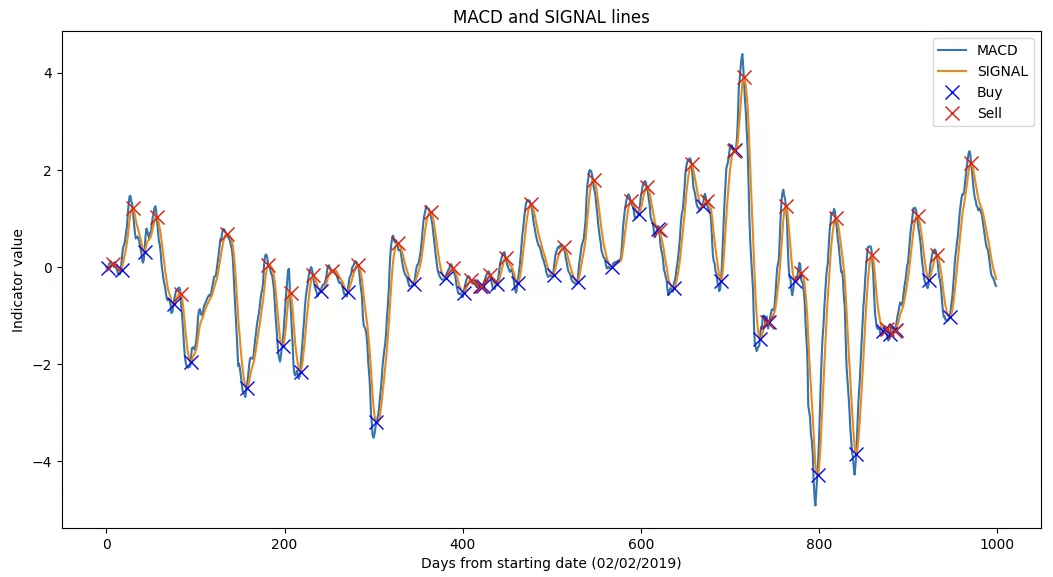
\includegraphics[width=0.9\textwidth]{macd.png}
  \caption{Wykres linii MACD oraz linii SIGNAL z naniesionymi punktami kupna/sprzedaży}
\end{figure}

\begin{figure}[h!]
  \centering
  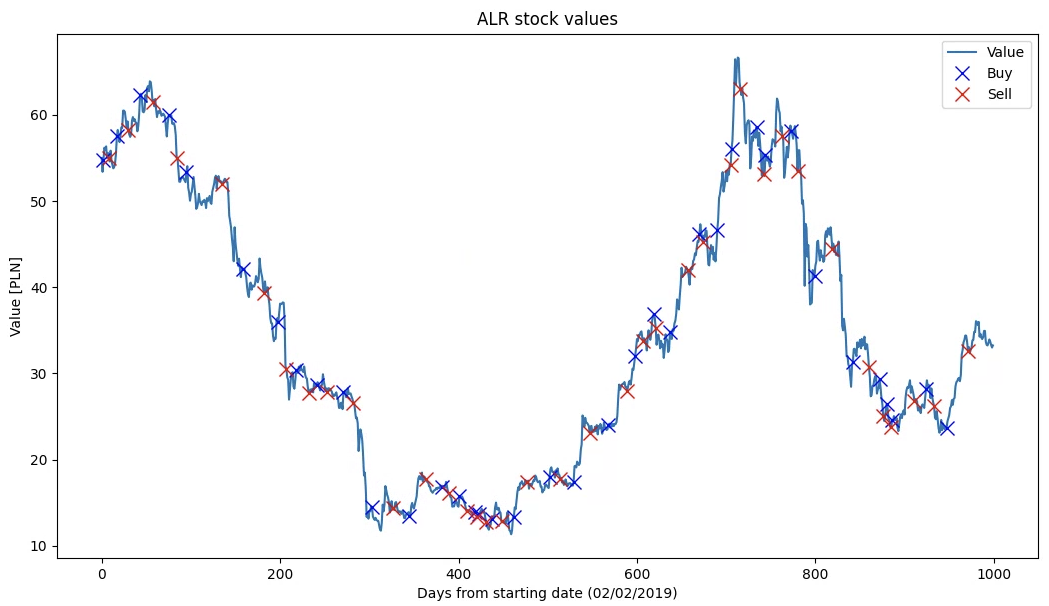
\includegraphics[width=0.9\textwidth]{values.png}
  \caption{Wykres wartości akcji ALR z naniesionymi punktami kupna/sprzedaży}
\end{figure}

\newpage

Sygnały do zakupu i sprzedaży akcji naniesione na wykres wartości akcji w formie znaczników potwierdzają fakt, że sygnały wyznaczane przez wskaźnik MACD są sygnałami opóźnionymi. Dzieje się tak dlatego, że wskaźnik ten dysponuje wyłącznie danymi historycznymi i reaguje jedynie na zmiany trendu (Rys. 3.a)). 

Ponadto wskaźnik MACD często zbyt nagle reaguje na chwilowe, krótkie zmiany kursu, przez co zdarzają się momenty, w których podczas silnego, lecz stałego trendu potrafi kilka razy z rzędu generować sygnały o zakupie/sprzedaży, gdy lepszą decyzją było cierpliwe przeczekanie (Rys. 3.b)). 

\begin{figure}[h!]%
    \centering
    \subfloat[\centering sygnały opóźnione]{{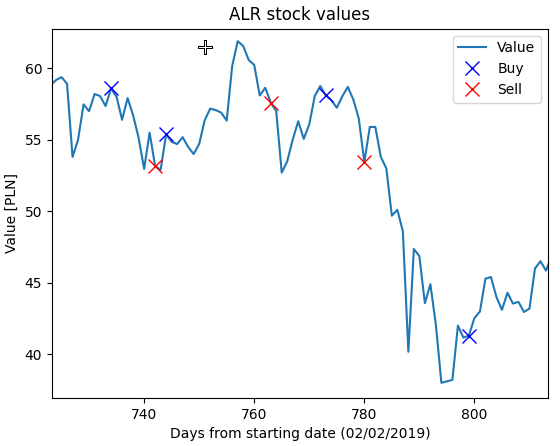
\includegraphics[width=8cm]{rys1.png} }}%
    \qquad
    \subfloat[\centering zbyt nagłe reakcje]{{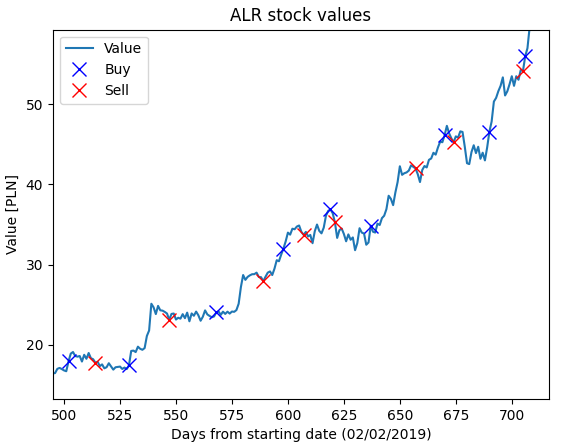
\includegraphics[width=8cm]{rys2.png} }}%
    \caption{Przykłady nieoptymalnych przypadków szczególnych}%
    \label{fig:example}%
\end{figure}

\subsection{Symulacja inwestycji na podstawie sygnałów wskaźnika}

W celu stwierdzenia przystosowania wskaźnika MACD do inwestycji, została przeprowadzona symulacja inwestycji. Inwestycja trwała przez cały okres, czyli przez tysiąc dni. Algorytm odpowiedzialny za kupno/sprzedaż akcji reagował na sygnały wskaźnika, kupując/sprzedając największą możliwą ilość akcji, biorąc pod uwagę obecny kapitał. W implementacji wzięto pod uwagę fakt, że akcje kupowane są w całości, to znaczy, że ilość kupionych akcji danego dnia musi być liczbą całkowitą. Jeżeli ostatniego dnia zostajemy z akcjami, algorytm je sprzedaje za cenę w ostatnim dniu.

\vspace{0.75em}
\begin{lstlisting}[language=Python, caption=Implementacja symulacji inwestycji z użyciem sygnałów wskaźnika MACD]
def simulateProfits(start, days, values, buy_days, sell_days):
    balance = start
    shares = 0
    for day in range(0, days):
        if buy_days[day]:
            shares = balance // values[day]
            balance -= shares * values[day]
        if sell_days[day]:
            balance += shares * values[day]
            shares = 0
    if shares != 0:
        balance = shares * values[days - 1]
    return balance - start
\end{lstlisting}
\vspace{0.5em}

Kapitał początkowy, który został zainwestowany, wynosił 1000 PLN. Po przeprowadzeniu symulacji uzyskano przychód w wysokości 776,65 PLN, co daje około 78\% zysku.

Końcowa cena akcji po 1000 dniach od pierwszej próbki była znacznie niższa od początkowej. Algorytm wykorzystując wskaźnik MACD uzyskał wysoki zysk. W okresie ok. od 100 do 300 dnia od pierwszej próbki ceny akcji diametralnie spadły, przez co algorytm stracił bardzo dużo kapitału, reagując na małe zmiany trendu. Pomimo dużych strat, algorytm poprawnie wykorzystał równie duży wzrost cen w okresie ok. od 500 do 700 dnia od pierwszej próbki.

\newpage
\section{Wnioski}

Wskaźnik giełdowy MACD dobrze nadaje się do analizy technicznej. Może być interpretowany na wiele różnych sposobów. Efektywnie informuje o zmianach trendów nie tylko przecięciami linii wskaźnika, ale też przecięciami zera i odległością między liniami MACD a SIGNAL \cite{web:trading_interpretation}. 

Wskaźnik MACD z powodu reakcji na najmniejsze zmiany trendu jest przydatny głównie do inwestycji długoterminowych, ponieważ przez dłuższy okres małe wahania tracą na ważności. Poza tym, wskaźnik ten nie nadaje się do analizy kursów, które cechują się dużymi wahaniami.

Algorytm inwestujący na podstawie sygnałów ze wskaźnika mógłby być usprawniony, gdyby po wykryciu dłuższego trendu rosnącego ograniczył swoje nagłe reakcje na nieistotne zmiany trendu, to znaczy na liczne przecięcia linii podczas trendu. To samo można zastosować w przypadku dłuższego trendu spadkowego, ograniczając bezsensowne zakupy akcji, które zostały sprzedawane chwilę później żeby ograniczyć straty.

\bibliographystyle{plain}
\bibliography{sample}

\end{document}